% !TeX spellcheck = es_ES
%%%%%%%%%%%%%%%%%%%%%%%%%%%%%%%%%%%%%%%%%
% Stylish Article
% LaTeX Template
% Version 2.1 (1/10/15)
%
% This template has been downloaded from:
% http://www.LaTeXTemplates.com
%
% Original author:
% Mathias Legrand (legrand.mathias@gmail.com) 
% With extensive modifications by:
% Vel (vel@latextemplates.com)
% Final ACS by:
% Juan Barbosa
% License:
% CC BY-NC-SA 3.0 (http://creativecommons.org/licenses/by-nc-sa/3.0/)
%
%%%%%%%%%%%%%%%%%%%%%%%%%%%%%%%%%%%%%%%%%
\documentclass[fleqn,10pt]{SelfArx}
%\usepackage[superscript]{cite}
\usepackage{wrapfig}
\usepackage{multirow}
%----------------------------------------------------------------------------------------
%	ARTICLE INFORMATION
%----------------------------------------------------------------------------------------

\JournalInfo{Laboratorio de Bioquímica, 07/02/2019} % Journal information
\Archive{ }

\PaperTitle{Aislamiento y determinación de ácidos nucleicos} %
%\Keywords{Keyword1 --- Keyword2 --- Keyword3} % Keywords - if you don't want any simply remove all the text between the curly brackets
%\newcommand{\keywordname}{Keywords} % Defines the keywords heading name

%----------------------------------------------------------------------------------------
%	ABSTRACT
%----------------------------------------------------------------------------------------

\Abstract{
}

%----------------------------------------------------------------------------------------

\begin{document}

\flushbottom % Makes all text pages the same height

\maketitle % Print the title and abstract box
%\tableofcontents % Print the contents section

\thispagestyle{empty} % Removes page numbering from the first page



%----------------------------------------------------------------------------------------
%	ARTICLE CONTENTS
%----------------------------------------------------------------------------------------

\section*{Introducci\'on} % The \section*{} command stops section numbering
%------------------------------------------------
	
\section{Secci\'on experimental}
	
\section{Resultados y Discusi\'on}
	\subsection{Aislamiento del ARN de levadura}
		Al disolver la levadura comercial en agua a una temperatura de 37 $^\circ$C se busca activar el metabolismo del hongo, para que esto pueda suceda es necesario que el organismo produzca ARN con el fin de iniciar la producci\'on de prote\'inas. En este sentido el control de la temperatura debe ser estricto, dado que cambios aumentos abruptos en esta, pueden llevar a que el organismo muera y cese su producci\'on del ARN que posteriormente ser\'a cuantificado.
		
		La adici\'on de fenol permite extraer los \'acidos nucl\'eicos de la levadura dada la polaridad del mismo. Los \'acidos nucl\'eicos debido a sus grupos fosfatos, constituyen mol\'eculas polares, las cuales se disuelven mejor en agua que en fenol. El proceso contrario sucede con las prote\'inas, las cuales tender\'an a estar en la fase org\'anica. La centrifugaci\'on de esta mezcla permite realizar la separaci\'on de fases, en donde en la fase acuosa se obtienen mayormente \'acidos nucl\'eicos y prote\'inas desnaturalizadas. La siguiente centrifugaci\'on permite aislar los \'acidos nucl\'eicos de las prote\'inas desnaturalizadas.
		
		Finalmente, y con el objetivo de precipitar los \'acidos nucl\'eicos se adiciona acetato de potasio y etanol, los cuales promueven la formaci\'on de enlaces entre los aniones de los grupos fosfatos de los \'acidos nucl\'eicos, y el ion potasio, con lo cual se neutraliza la mol\'ecula, ocasionando su precipitaci\'on.
		
		
%		 If the aim of an experiment is to obtain samples of purified RNA, a pH of around 4.5 is used. Because of the negative charge on the backbone of DNA from phosphates, decreasing the pH of a solution will lead to neutralization. A pH of 4.5 has a higher concentration of H+ ions that would neutralize the negative phosphate charges and cause DNA to dissolve in the organic phase, while RNA has additional hydroxyl group in pentose sugar which allows the RNA to remain in water phase. 
%		\cite{toni2018optimization}
		
	\subsection{Aislamiento del ADN de fresa}
	
	\subsection{Cuantificaci\'on de \'acidos nucl\'eicos}
		Se debe tener en cuenta que en el caso del ARN de la \textit{S. cerevisiae} un contaminante com\'un que puede aumentar las lecturas de absorbancia en 280 nm es el fenol, el cual absorbe en cerca de 270 nm y pudo haber permanecido en la muestra luego del proceso de extracci\'on \cite{toni2018optimization}.
		
	\begin{figure*}[h]
		\centering
		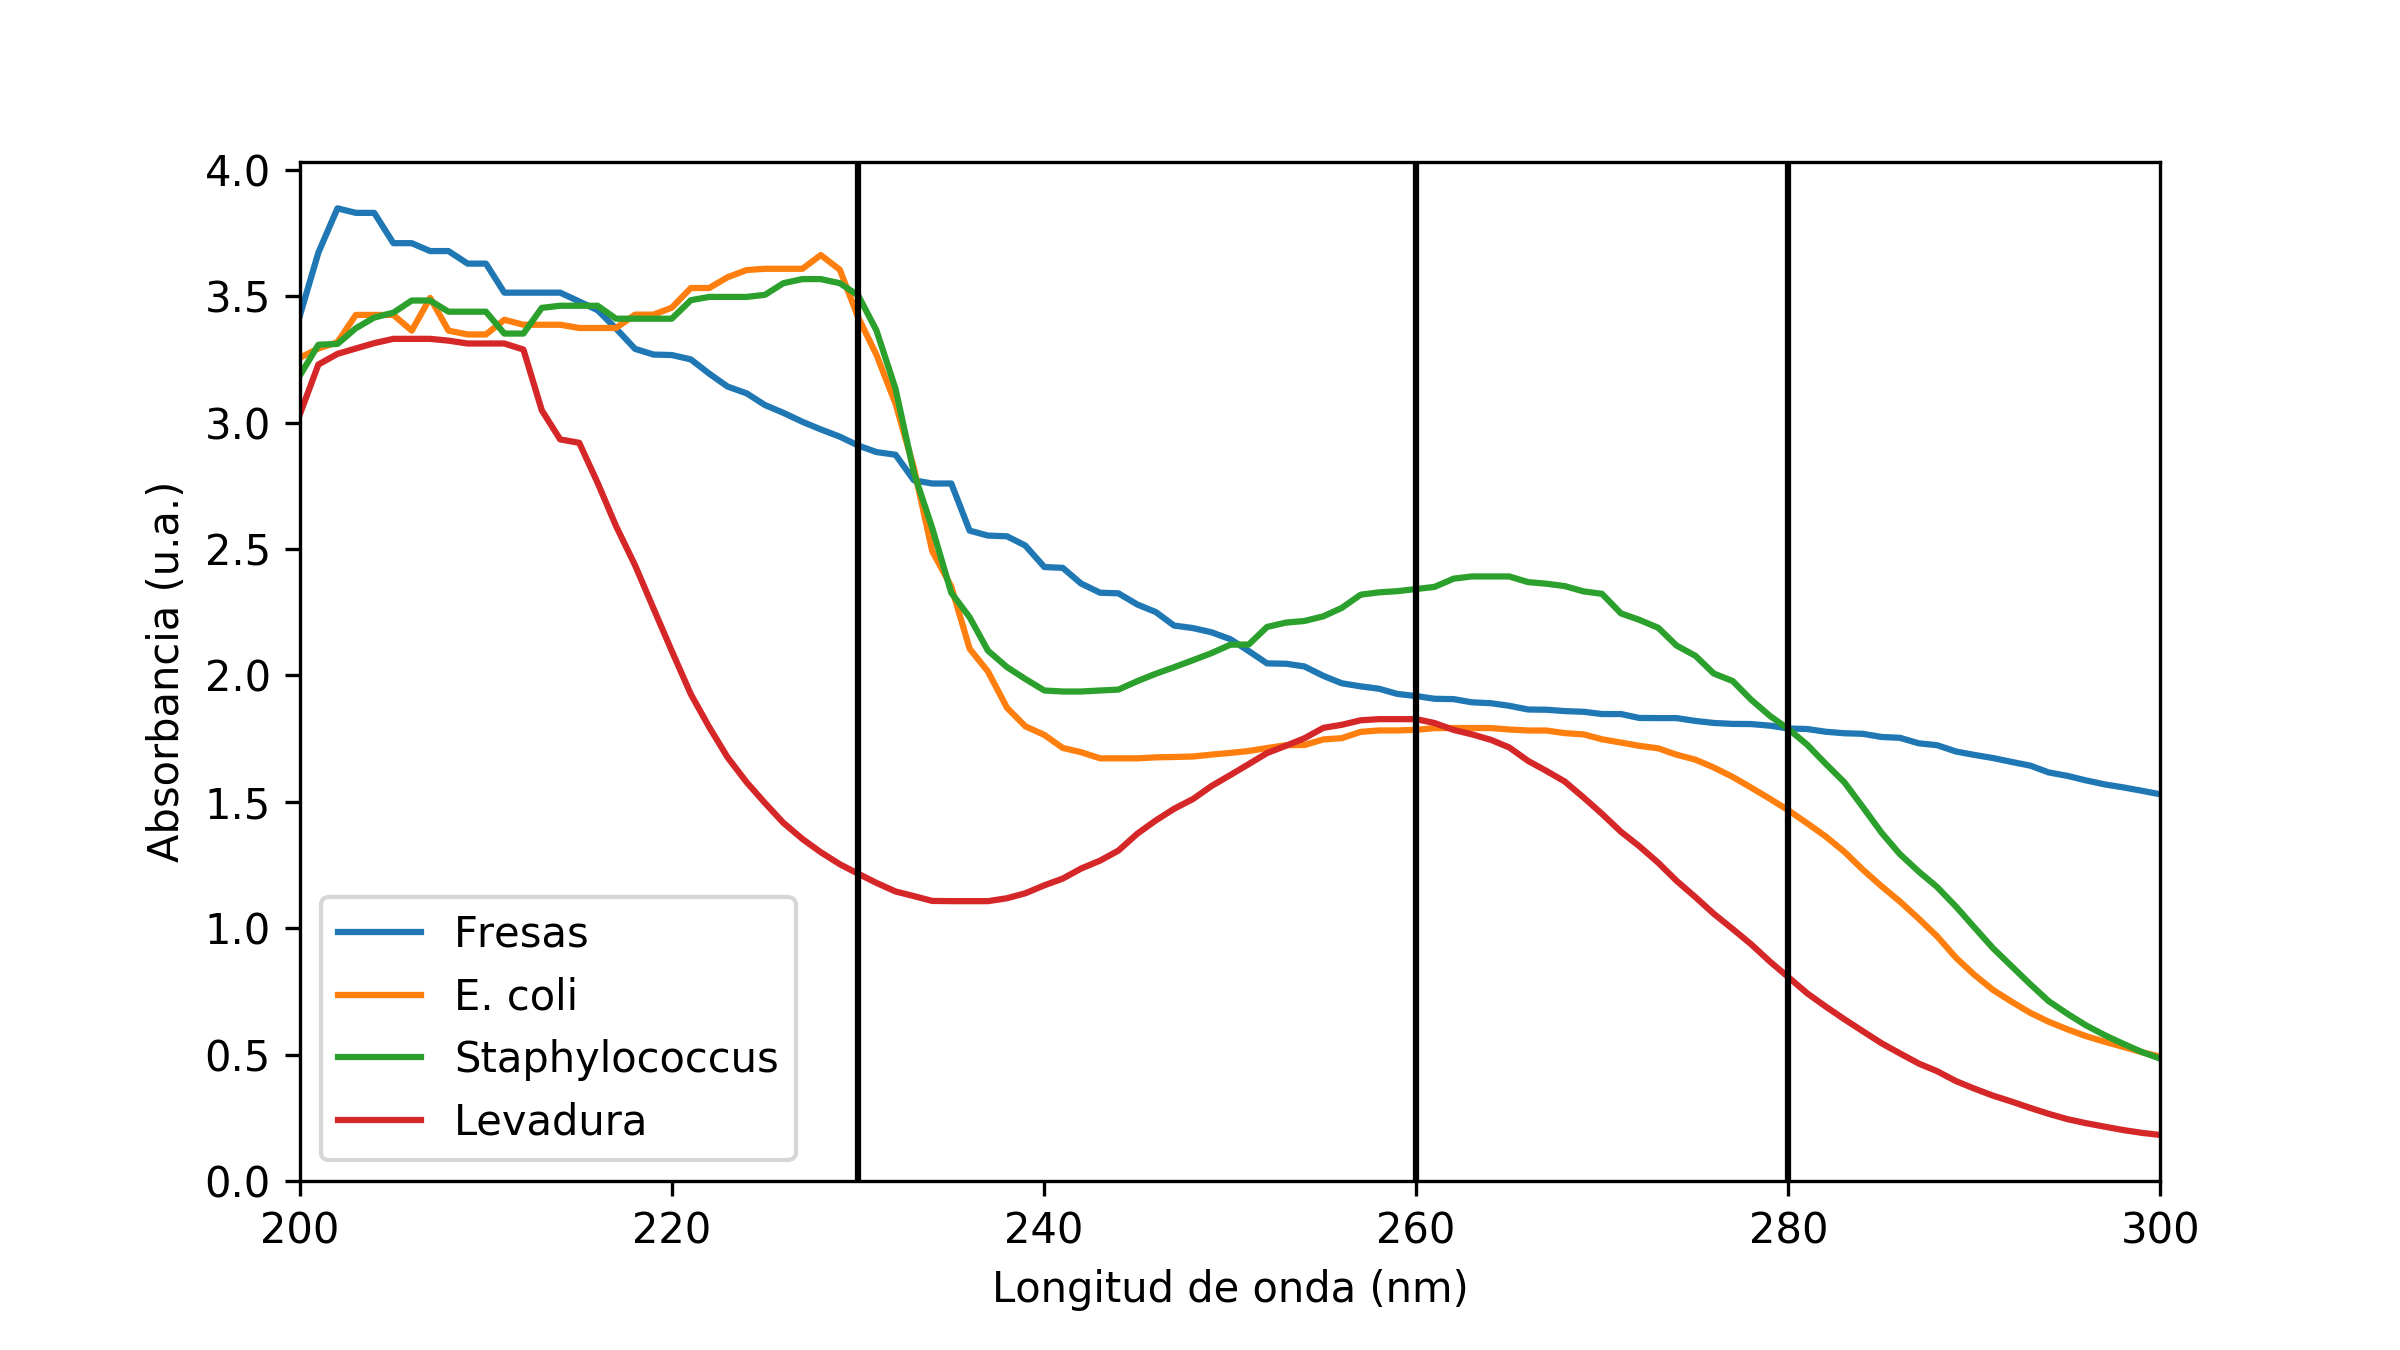
\includegraphics[width=\linewidth]{plots}
		\caption{Absorbancias obtenidas para las distintas muestras en funci\'on de la longitud de onda.}
	\end{figure*}

	\begin{table}[h]
		\centering
		\caption{Absorbancias a 230, 260 y 280 nm (u.a.), junto con la relaci\'on 260/280.}
		\begin{tabular}{c|ccc|c}
			\hline
			\textbf{Muestra} & $A_{230}$ & $A_{260}$ & $A_{280}$ & $A_{260} / A_{280}$ \\
			\hline
			\textit{F. ananassa} & 2.97 & 1.91 & 1.79 & 1.06 \\
			\textit{E. coli} & 4.85 & 1.79 & 1.47 & 1.22 \\
			\textit{S. aureus} & 3.50 & 2.35 & 1.79 & 1.31 \\
			\textit{S.cerevisiae} & 1.22 & 1.83 & 0.81 & 2.27 \\
			\hline
		\end{tabular}
	\end{table}
	\cite{sambrook2001molecular}
\section{Conclusiones}
	
%----------------------------------------------------------------------------------------
%	REFERENCE LIST
%----------------------------------------------------------------------------------------
\phantomsection
\bibliography{informe}
\bibliographystyle{unsrt}

%----------------------------------------------------------------------------------------
%\newpage
%\onecolumn
%\section{Informaci\'on suplementaria}\label{sec: complementaria}
\end{document}